%%
%% Template conclusion.tex
%%

\chapter{Discussion}
\label{cha:Discussion}
In this chapter, we first proposed a road scene understanding approach that worked well in our experiments. Then, we compared two unsupervised learning methods (convolutional auto-encoders and PCA), and analyzed the applicability of super-pixel denoising. After that, we discussed the limitations of our study and stressed out potential future works.

\section{Best Practice}
It is shown in Figure \ref{resfig} that, convolutional auto-encoders based methods yielded the best result in our experiment settings. If super-pixel labeling was applied in the inference step, we could further improve the perdition accuracy by approximately $0.5\%$. Therefore our best choice would be to use convolutional auto-encoders to pre-train on unlabeled data, then use the trained parameters to initialize a convolutional neural network, and use super-pixel labeling for inferring the labels of an input image. 

In the best case, this approach gives an accuracy of $89.51\%$ on noiseless test data, which exceeds the baseline by $2.7\%$. When trained on the data set with a noise ratio of $12.74\%$, it can reach a same noise level ($12.67\%$) as of the training data, hence shows its robustness to noise. A comparison of prediction results and generated labels are shown is Figure \ref{noisefig}, as we can see, the prediction result of our approach looks better than the generate labels in this case.

\begin{figure}[h!]
\centering
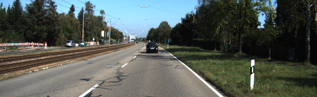
\includegraphics[width=0.7\linewidth]{pics/img.png}

\includegraphics[width=0.7\linewidth]{pics/super.png}

\includegraphics[width=0.7\linewidth]{pics/noise.png}
\caption{Example of an input image (top), prediction result (middle), and generated labels (down). }
\label{noisefig}
\end{figure}

We can know from comparing Table \ref{mantab} and \ref{supertab}, when trained on a small amount of data, the advantage of unsupervised feature learning using convolutional auto-coders becomes more noticeable, which confirms the effectiveness of convolutional auto-coders in leveraging the usability of unlabeled data. 

Moreover, better results were obtained when trained on noiseless data than noisy data, even if the amount of data set is much smaller (40 images vs. 264 images). Therefore we believe out performance can be further improved given sufficient amount of well labeled data.

An other benefit of this approach is, its running time in the prediction stage becomes linear with respect to the size of input data. If the network architecture is fixed, its time complexity will only be dominated by the time of performing image segmentation algorithms. Moreover, it is traceable in the sense that we can control its running time by adjusting the network architecture and the number of super-pixels, at the expense of accuracy. 

Linear and tractable running time is a desirable property in real world applications. For example, in autonomous driving systems, we want to reduce the running time to the minimum since our surrounding environment can change rapidly. Some algorithms for high level handcrafted features are of superlinear time complexity, which constrains their practical utility.

\section{Convolutional Auto-encoders vs. Principal Component Analysis}
As shown in our experiment results, PCA could also produce comparable outputs to convolutional auto-encoders. However convolutional auto-encoders have shown their advantages in many aspects. Convolutional auto-encoders provide us insight into how to adjust the architecture of neural networks. It learns local features instead of global features, which is a more reasonable approach for image data. In the prediction stage, convolutional auto-encoders can be used directly on input data, while PCA require a pre-processing operation.

In terms of computational resources, the memory requirement for training convolutional auto-encoders is independent of the size of input data if online optimization algorithms are used (e.g., stochastic gradient decent). On the other hand, PCA is often subject to high space complexity when performed on high resolution images. For instance, for a 1024 by 1024 color image, the size of the covariance involved will be $(1024\times1024\times3)^2$, which will take terabytes of memory. Although algorithms such as partial least squares~\cite{geladi1986partial} can be used to approximate PCA, they are of their own limitations.

\section{Super-pixel Denoising}
Although the Markov random fields can be used for noise reduction on a super-pixel level in many cases, it has a serious drawback. The assumption that a strong correlation exists between adjacent super-pixels does not hold in general. For instance, in the case that a pedestrian (represented by a super-pixel) on the road has been predicted successfully into the ``object'' category, because its surrounding area has been labeled as ``road'', using MRF denoising will turn the label of that pedestrian super-pixel into the same category as its neighbours. More importantly such misclassifications will cause safety issues if applied on autonomous driving systems, hence MRF denoising is not considered as a beneficial method for our purpose.

\section{Limitations and Future Work}
We have analyzed the pros and cons of various methods, and suggested a weakly supervised method which is of acceptable accuracy, tractable running time and is robust to noise. On the other hand, there are several limitations of our study. 

First, because we did not have an adequate amount of well labeled data, we can not give a performance upper bound of this approach. Second. our experiment was conducted using data from the same source (KITTI Road data set). Its generalizability on other data sets has not been tested. Third, because we used fixed size patches as input data, in some cases a patch does not contain enough information for inferring the label of the centering pixel [reflection pic]. Another aspect we chose to neglect in our study is the relationship between consecutive images in a video.
 
In the next step, we will first focus on addressing the data issues mentioned above. Then we are going to investigate techniques for capturing the global information of an image and the correlation between consecutive images. Furthermore, we may want to explore a more complex road scene understanding task. For instance, we can add more categories denoting pedestrians, vehicles, and side walks.